\begin{figure}[t]
\centering
% Vector drawing generated by tools/figures/build.py; rerun it after changing the figure.
\ifbilingual
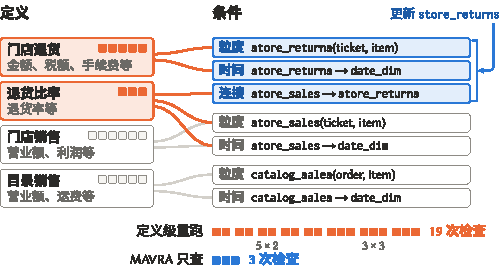
\includegraphics[width=\linewidth]{figures/sharing-zh}
\else
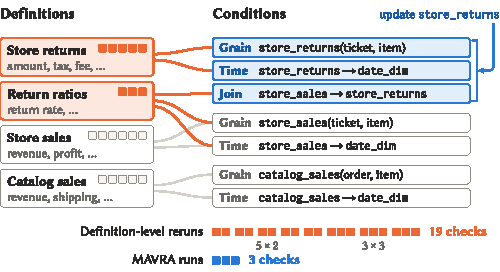
\includegraphics[width=\linewidth]{figures/sharing}
\fi
\caption{\bt{Definitions share conditions. The 19 definitions of the controlled workload reference 41 condition instances but only seven distinct conditions. After an update of \code{store\_returns}, the eight definitions on orange edges become pending.}{定义共享条件。受控负载的 19 个定义引用 41 个条件实例，但不同的条件只有 7 个。\code{store\_returns} 更新后，橙色边上的 8 个定义变为待验证。}}
\label{fig:sharing}
\Description{Four definition families on the left, drawn as cards with one tile per definition: store returns (5), return ratios (3), store sales (6), and catalog sales (5). Seven conditions on the right; the three that read store\_returns are highlighted and marked as touched by an update of store\_returns. Orange edges connect the eight pending definitions to every condition they reference. Below, definition-level revalidation reruns 19 checks, five definitions times two plus three times three, whereas MAVRA runs three.}
\end{figure}
